\documentclass[aspectratio=169, t, 8pt]{beamer}

%------configurando acentos-----------
\usepackage[utf8]{inputenc}
\usepackage[T1]{fontenc}
\usepackage[brazil]{babel}
\usepackage{montserrat}
\usefonttheme[onlymath]{serif}
\usepackage{booktabs} % Tabelas elegantes sem linhas verticais
\usepackage{multirow}
\usepackage{array}
\usepackage[most]{tcolorbox}
\usepackage{graphicx}
% \usepackage[inline]{enumitem}

\DeclareMathOperator{\sen}{sen}

%-------Estilos Beamer---------------
\usetheme{metropolis}
%\usecolortheme{crane}
%\usefonttheme{serif}
\linespread{1.2}

% Personalização de Cores (Exemplo: Minimal Teal)
% Cores Base
\definecolor{BgCanvas}{HTML}{F9F9FB}      % Off-white muito suave
\definecolor{MainText}{HTML}{2B2D42}      % Grafite escuro para alta legibilidade
\definecolor{PrimaryAccent}{HTML}{4A6FA5} % Azul poeira (Dusty Blue)

% Tons Pastéis para Destaques e Cards
\definecolor{PastelGreenBg}{HTML}{E8F0EC}  % Sálvia Claro (Sucesso / Destaque Positivo)
\definecolor{PastelGreenFg}{HTML}{2D5A44}

\definecolor{PastelCoralBg}{HTML}{FDEAE6}  % Coral Soft (Atenção / Problema / Alerta)
\definecolor{PastelCoralFg}{HTML}{7A3025}

\definecolor{PastelPurpleBg}{HTML}{F0EBF4} % Lavanda (Conceitos / Citações)
\definecolor{PastelPurpleFg}{HTML}{4A3E56}

\definecolor{PastelYellowBg}{HTML}{FFF4E6} % Areia / Manteiga (Notas / Dados Secundários)
\definecolor{PastelYellowFg}{HTML}{7A522A}

% --- CONFIGURAÇÕES DE TEMA BEAMER ---
%\usetheme{metropolis}

\setbeamertemplate{itemize item}{\textcolor{MainText}{$\bullet$}}
\setbeamertemplate{itemize subitem}{\textcolor{MainText}{\scriptsize$\circ$}}
\setbeamertemplate{itemize 3rditem}{\textcolor{MainText}{\tiny$\blacksquare$}}

\setbeamercolor{background canvas}{bg=BgCanvas}
\setbeamercolor{normal text}{fg=MainText}
\setbeamercolor{frametitle}{bg=PastelGreenFg, fg=BgCanvas}
\setbeamercolor{title}{fg=MainText}
\setbeamercolor{subtitle}{fg=PrimaryAccent}
\setbeamercolor{structure}{fg=PrimaryAccent}

% Remove a linha amarela padrão do Metropolis sob o título
\setbeamertemplate{title separator}{}
\setbeamertemplate{progress bar in section page}{}

% ==============================================================================
% PALETA DE CORES "GEOMETRIA AQUECIDA" (Inspirada na imagem)
% ==============================================================================
\definecolor{BgCream}{HTML}{FFFDFB}       % Fundo creme suave
\definecolor{TextDark}{HTML}{2C1A14}      % Texto em castanho escuro elegante
\definecolor{PrimaryOrange}{HTML}{E0531C}  % Laranja vibrante (Títulos e destaques)
\definecolor{Terracotta}{HTML}{B8380D}     % Terracota queimado (Alertas)
\definecolor{SoftOrange}{HTML}{FFE6D5}     % Laranja bem suave (Fundo de blocos)

% =================================================
% CONFIGURAÇÃO DO TEMA METROPOLIS
% =================================================
% Cores do texto e fundo geral
\setbeamercolor{normal text}{fg=TextDark, bg=BgCream}
\setbeamercolor{alerted text}{fg=Terracotta}
\setbeamercolor{example text}{fg=PrimaryOrange}

% Barra de título dos slides (Frametitle)
\setbeamercolor{frametitle}{fg=BgCream, bg=PrimaryOrange}

% Título principal da apresentação (Slide de Capa)
\setbeamercolor{titlelike}{fg=PrimaryOrange}
\setbeamercolor{subtitle}{fg=Terracotta}

% Barra de progresso (Linha do Metropolis)
\setbeamercolor{progress bar}{fg=PrimaryOrange, bg=PrimaryOrange!20}

% Customização de Blocos (block, alertblock, exampleblock)
\setbeamercolor{block title}{fg=BgCream, bg=PrimaryOrange}
\setbeamercolor{block body}{fg=TextDark, bg=SoftOrange}

\setbeamercolor{block title alerted}{fg=BgCream, bg=Terracotta}
\setbeamercolor{block body alerted}{fg=TextDark, bg=Terracotta!15}


% --- ESTILOS DE CARDS PASTEL COM TCOLORBOX ---
\newtcolorbox{cardPrincipal}[1][]{
  colback=SoftOrange,
  colframe=Terracotta,
  coltext=TextDark,
  arc=6pt,
  boxrule=0pt,
  left=12pt, right=12pt, top=10pt, bottom=10pt,
  fonttitle=\bfseries\small,
  #1
}

\newtcolorbox{cardcoral}[1][]{
  colback=PastelCoralBg,
  colframe=PastelCoralFg,
  coltext=PastelCoralFg,
  arc=6pt,
  boxrule=0pt,
  left=12pt, right=12pt, top=10pt, bottom=10pt,
  fonttitle=\bfseries\small,
  #1
}

\newtcolorbox{cardpurple}[1][]{
  colback=PastelPurpleBg,
  colframe=PastelPurpleFg,
  coltext=PastelPurpleFg,
  arc=6pt,
  boxrule=0pt,
  left=12pt, right=12pt, top=10pt, bottom=10pt,
  fonttitle=\bfseries\small,
  #1
}

\newtcolorbox{cardyellow}[1][]{
  colback=PastelYellowBg,
  colframe=PastelYellowFg,
  coltext=PastelYellowFg,
  arc=6pt,
  boxrule=0pt,
  left=12pt, right=12pt, top=10pt, bottom=10pt,
  fonttitle=\bfseries\small,
  #1
}

\graphicspath{{../../src/img/semana06/}}

%--------Dados do Documento
\title{Geometria: Trigonometria}
\subtitle{}
\author{prof. Eduardo}
\institute{Pré-Universitário Oficina do Saber / UFF}

\date{\today}


%-------- Pacotes Matemática -------------
\usepackage{amsmath}
\usepackage{amsthm}
\usepackage{amsfonts}
\usepackage{amssymb}
\usepackage{xfrac}
\usepackage{thmtools}

\begin{document}

    \begin{frame} %capa
        \vspace*{\fill}
            
            \begin{columns}[c]
                \begin{column}{0.5\textwidth}
                    {\usebeamerfont{title}\usebeamercolor[fg]{title}\inserttitle}\vspace{0.2cm}
                    
                    {\usebeamerfont{subtitle}\usebeamercolor[fg]{subtitle}\insertsubtitle}\vspace{0.5cm}

                {\usebeamerfont{author}\insertauthor}\vspace{0.3cm}

                {\usebeamerfont{institute}\insertinstitute}\vspace{0.3cm}

                {\usebeamerfont{date}\insertdate}
            \end{column}
            
            
            \begin{column}{0.4\textwidth}
                \centering
                
\includegraphics[width=0.4\textwidth]{../logo_ofSaber.png}

                \vspace{.4cm}
                \vspace*{\fill}
        \begin{columns}[c]
            \begin{column}{.5\textwidth}
                \centering
\includegraphics[width=.5\textwidth]{../Proex02c.png}
            \end{column}
            \begin{column}{.5\textwidth}
                \centering
\includegraphics[width=0.4\textwidth]{../Logo_UFF.png}
            \end{column}
        \end{columns}
        \vspace*{\fill}
            \end{column}
        \end{columns}
    \vspace*{\fill}
    \end{frame}
    
        % {
        %     \usebackgroundtemplate{
        %     
\includegraphics[width=\paperwidth]{segunda_capa_pitagoras.png}}
        %     \begin{frame}[plain]                
        %     \end{frame}
        % }

    % \begin{frame}{Ângulos}
    %     \begin{columns}[T]
    %         \begin{column}{0.4\textwidth}
    %             \begin{cardPrincipal}[title=Ângulo]
    %                 Definimos ângulo geométrico como a reunião de duas semi-retas com um ponto de origem em comum.
    %             \end{cardPrincipal}
    %             \begin{figure}
    %                 \centering
    %                 
\includegraphics[width=.9\textwidth]{angulos_interno_externo.jpeg}
    %             \end{figure}
    %         \end{column}
    %         \begin{column}{.55\textwidth}
    %             \vspace{1em}
    %             A região interna de um ângulo é chamada \textbf{ângulo interno}, enquanto a região externa é denominada ângulo externo.

    %             Normalmente, ao nos referirmos a um ângulo, estamos tratando de dua região interna.

    %             Para referenciarmos o ângulo ao lado, utilizamos as seguintes notações:

    %             {
    %                 \centering
    %                 \[
    %                     \widehat{AOB} \quad \text{\textbf{ou}} \quad A\hat{O}B
    %                 \]
    %             }

    %             O ponto $O$ é chamado \textbf{vértice} do ângulo.

    %             As unidades de medida mais comuns são o \textbf{grau}($^\circ$) ou o \textbf{radiano}($rad$).

    %             Um grau é a divisão de uma circunferência em 360 partes. Enquanto o radiano se relaciona ao raio da circunferência. Nesta aula, utilizaremos somente o grau.
    %         \end{column}
    %     \end{columns}    
    % \end{frame}

    % \begin{frame}{Classificação de Ângulos}
    %     \centering
    %     \begin{tabular}{p{.2\linewidth} p{.2\linewidth} p{.2\linewidth} p{.2\linewidth}}
    %         \toprule
    %         \textbf{Agudo} & \textbf{Reto} & \textbf{Obtuso} & \textbf{Raso}\\
            
    %         \midrule
            
    %         
\includegraphics[width=.2\columnwidth]{angulo_agudo.jpeg} & 
\includegraphics[width=.2\columnwidth]{angulo_reto.jpeg} & 
\includegraphics[width=.2\columnwidth]{angulo_obtuso.jpeg} & 
\includegraphics[width=.2\columnwidth]{angulo_raso.jpeg}\\

    %         \midrule

    %         é o angulo de medida \textbf{menor} que 90° & é o angulo de medida \textbf{igual} a 90° & é o angulo de medida \textbf{maior} que 90° & é o angulo de medida \textbf{igual} a 180°\\
            
    %         \bottomrule
    %     \end{tabular}
    %     \vspace{1em}
    %         \begin{columns}[T]
    %             \begin{column}{0.4\textwidth}
    %                \begin{cardPrincipal}[title=Ângulos Complementares]
    %                     Um ângulo $\hat{B}$ é complementar a um ângulo $\hat{A}$, se: $\hat{A} + \hat{B} = 90^\circ$
    %                \end{cardPrincipal}
    %             \end{column}
    %             \begin{column}{0.4\textwidth}
    %                 \begin{cardPrincipal}[title=Ângulos Suplementares]
    %                     Um ângulo $\hat{B}$ é complementar a um ângulo $\hat{A}$, se: $\hat{A} + \hat{B} = 180^\circ$
    %                \end{cardPrincipal}
    %             \end{column}
    %         \end{columns}
    % \end{frame}    

    % \begin{frame}{Triângulos: Definição e Classificação}
    %     Triângulos são polígonos que possuem três vértices, três lados e três ângulos. A \textbf{soma das medidas dos ângulos internos} de qualquer triângulo é $180^\circ$. Eles podem ser classificados quanto a seus ângulos ou quanto a seus lados.

    %     \vspace{1em}

    %     \centering
    %     \begin{table}[h]
    %     \begin{tabular}{|m{0.02\linewidth} | p{0.2\linewidth} | p{0.3\linewidth} | p{0.3\linewidth}|}
    %         \hline
        
    %         \multirow{3}{*}{\rotatebox{90}{\textbf{Lados}}}   & \textbf{Equilátero}  & Seus lados possuem a mesma medida & Seu ângulos medem $60^\circ$. É um \textit{caso especial} do triângulo isósceles\\ 
            
    %         \cline{2-4} 
            
    %         & \textbf{Isósceles}   & Possui ao menos dois lados de mesma medida & Os ângulos de sua base são congruentes \\
            
    %         \cline{2-4} 
            
    %         & \textbf{Escaleno}    & Possui três lados diferentes      & Possui também três ângulos diferentes \\
            
    %         \hline
                    
    %         \multirow{3}{*}{\rotatebox{90}{\textbf{Ângulos}}} & \textbf{Acutângulo}  & Possui três ângulos agudos        & Será \textbf{Equiângulo} se seus ângulos medem ($60^\circ$) \\
            
    %         \cline{2-4} 
    %         & \textbf{Retângulo}   & Possui um ângulo reto & Seus outros ângulos são agudos \\
            
    %         \cline{2-4} 
    %         & \textbf{Obtusângulo} & Possui um ângulo obtuso & Seus outros ângulos são agudos \\
            
    %         \hline
    %     \end{tabular}
    % \end{table}
    % \end{frame}

    % \begin{frame}{Semelhança entre Triângulos}
    %     \centering
    %     \begin{columns}[T, totalwidth=.9\textwidth]
    %         \begin{column}{.3\textwidth}
    %             
\includegraphics[width=.85\textwidth]{semelhanca_de_triangulos.jpeg}
    %         \end{column}
    %         \begin{column}{.65\textwidth}
    %             Quando tratamos de semelhança entre triângulos, estamos falando de formato e não de tamanho. Portanto, a \textbf{igualdade entre os ângulos} de dois triângulos garante a semelhança.
                
    %             A igualdade entre os ângulos garante, portanto, que haja uma razão de semelhança entre os lados \textbf{homólogos}.

    %             Lados homólogos são os lados dois triângulos semelhantes que se opõem aos ângulos de mesmo valor. Se o triângulo é semelhante, os lados guardarão uma mesma \textbf{razão de semelhança}$\left( k \right)$.
    %             No caso ao lado:

    %             \[
    %                 \triangle ABC = \frac{1}{2} \triangle PQR \quad \therefore \quad k=\frac{1}{2} 
    %             \]

    %             Esses conceitos nos permitem estabelecer alguns procedimentos para analisarmos a semelhança entre triângulos.

    %         \end{column}
    %     \end{columns}
    % \end{frame}

    % \begin{frame}{Casos de Semelhança entre Triângulos}
    %     Temos, basicamente três casos de análise para determinarmos se dois triângulos são semelhantes ou não.

    %     \begin{tabular}{|p{.3\linewidth}|p{.3\linewidth}|p{.3\linewidth}|}
    %         \hline
    %         \textbf{Caso AA} & \textbf{Caso LLL} & \textbf{Caso LAL}\\
    %         \hline
    %         \textit{ângulo-ângulo} & \textit{lado-lado-lado} & \textit{lado-ângulo-lado}\\
    %         \hline
    %         Se dois triângulos possuem dois de seus ângulos congruentes, eles são semelhantes & Se dois triângulos possuem lados homólogos igualmente proporcionais, eles são semelhantes & Se dois triângulos possuem dois lados com medidas proporcionais e o ângulo formado por esses lados é congruente, então a semelhança entre os triângulos é garantida\\
    %         \hline 
    %     \end{tabular}
    % \end{frame}

    % \begin{frame}{Teorema de Pitágoras}
    %     \begin{columns}[T, totalwidth=.9\textwidth]
    %         \begin{column}{.4\textwidth}
    %             \centering
    %             
\includegraphics[width=.9\textwidth]{teorema_de_pitágoras.jpeg}
    %         \end{column}
    %         \begin{column}{.55\textwidth}
    %             A relação de igualdade entre a soma dos quadrados dos catetos e o quadrado da hipotenusa se observa para todos os triângulos retângulos.

    %             Esse teorema, um dos mais lindos e significativos da Matemática é herdeiro do conhecimento da semelhança entre triângulos.

    %             É atribuído a Pitágoras a demonstração e generalização do teorema. A relação entre determinados triângulos retângulos já eram conhecidos muito antes de Pitágoras na Babilônia e no Egito.

    %             Um dos principais usos se relaciona ao cálculo de distâncias. Por exemplo, para calcularmos altura de triângulos isósceles, distância entre dois pontos, etc.
    %         \end{column}
    %     \end{columns}
    % \end{frame}

    % \begin{frame}{Trigonometria}
    %     Um outro avanço foi proporcionado pela relação pitagórica e pela semelhança de triângulos: as funções seno, cosseno, tangente e suas variações.

    %     O que garante que elas "funcionam" é justamente a razão de semelhanças entre os lados dos triângulos retângulos. Se tomamos um ângulo como referência, a razão entre dois de seus lados será a mesma para qualquer triângulo semelhante.

    %     Sendo assim, o valor decimal que obtemos da divisão entre as medidas irá ser constante para o ângulo. É isso que nos possibilita escrever as funções tringonométricas em função dos valores dos ângulos.
    %     \begin{figure}
    %         \centering
    %         
\includegraphics[width=.8\textwidth]{trigonometria.png}
    %     \end{figure}
    % \end{frame}

%----------------------------------------------
%              EXERCICIOS
%----------------------------------------------

    \begin{frame} {Exercícios} %Gabarito B
        \begin{columns}
            \centering
            \begin{column}{.9\textwidth} %letra a
                1.~\textbf{(ENEM-2017): } Raios de luz solar estão atingindo a superfície de um lago formando um ângulo $x$ com a sua superfície, conforme indica a figura

                Em determinadas condições, pode-se supor que a intensidade luminosa desses raios, na superfície do lago, seja dada aproximadamente por $l(x)=k \cdot \sen{(x)}$, sendo $k$ uma constante e supondo-se que $x$ é um ângulo entre $0^\circ$ e $90^\circ$.
                Quando $x = 30^\circ$, a intensidade luminosa se reduz a qual percentual de seu valor máximo. 

                \vspace{1.2em}
                \centering
                \begin{columns}
                    \begin{column}{.65\textwidth}
                        \begin{figure}
                            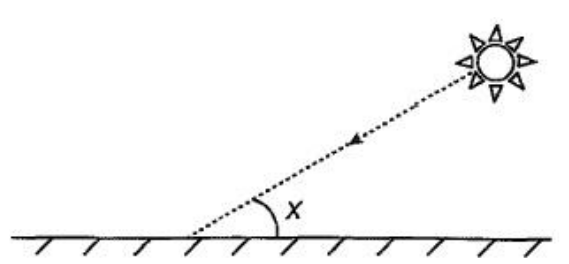
\includegraphics[width=.8\textwidth]{questao01.png}
                        \end{figure}
                    \end{column}
                    \begin{column}{.3\textwidth}
                        \begin{enumerate}[a.]
                            \item $33\%$
                            \item $50\%$
                            \item $57\%$
                            \item $70\%$
                            \item $86\%$
                        \end{enumerate}
                    \end{column}
                \end{columns}
            \end{column}
        \end{columns}
    \end{frame}

    % \begin{frame} %Gabarito D
    %     \frametitle{Exercícios}
    %     \begin{columns}
    %         \begin{column}{.9\textwidth}
    %             2.~\textbf{(UFRGS-1996): }APara estimar a profundidade de um poço com 1,10 m de largura, uma pessoa cujos olhos estão a 1,60 m do chão posiciona-se a 0,50 m de sua borda. Desta forma, a borda do poço esconde exatamente seu fundo, como mostra a figura.

    %             \begin{columns}
    %                 \begin{column}{0.3\textwidth}
    %                     \begin{figure}
    %                         \centering
    %                         
\includegraphics[width=\textwidth]{questao02.png}
    %                     \end{figure}
    %                 \end{column}
    %                 \begin{column}{0.65\textwidth}
    %                     \vspace{0.2cm}

    %                     A partir dos dados acima, podemos concluir que a profundidade do poço é:

    %                     \begin{enumerate}[a.]
    %                         \item 2,82 m
    %                         \item 3,00 m
    %                         \item 3,30 m
    %                         \item 3,52 m
    %                         \item 3,85 m
    %                         % letra e
    %                     \end{enumerate}

    %                 \end{column}
    %             \end{columns}
    %         \end{column}
    %     \end{columns}
    % \end{frame}

    % \begin{frame} %Exercício 03
    %     \frametitle{Exercícios}
    %     \begin{columns}
    %         \begin{column}{.9\textwidth}
    %             3.~\textbf{(UNESP-1997): }Na figura, $B$ é um ponto do segmento de reta $\overline{AC}$ e os ângulos $\widehat{DAB}$, $\widehat{DBE}$ e $\widehat{}{BCE}$ são retos.
              
    %             \begin{columns}
    %                 \begin{column}{0.6\textwidth}
    %                     \begin{table}
    %                         \begin{figure}
    %                             \centering
    %                             
\includegraphics[width=\textwidth]{questao03.png}
    %                         \end{figure}
    %                     \end{table}
    %                 \end{column}
    %                 \vspace{1em}
    %                 \begin{column}{0.35\textwidth}
    %                     Se o segmento $\overline{AD} = 6\text{ dm}$, o segmento $\overline{AC}=11\text{ dm}$ e o segmento $\overline{EC}=3\text{ dm}$, as medidas possíveis de $\overline{AB}$, em dm, são:
    %                     \vspace{1.2em}
    %                     \begin{enumerate}[a.]
    %                         \item 4,5 e 6,5
    %                         \item 7,5 e 3,5
    %                         \item 8 e 3
    %                         \item 7 e 4
    %                         \item 9 e 2
    %                         % letra E
    %                     \end{enumerate}

    %                 \end{column}
    %             \end{columns}
    %         \end{column}
    %     \end{columns}
    % \end{frame}

    % \begin{frame} %Exercicio 04
    %     \frametitle{Exercícios}
    %     \begin{columns}
    %         \begin{column}{.9\textwidth}
    %             4.~\textbf{(UNIRIO-1998): }Numa cidade do interior, à noite, surgiu um objeto voador não identificado, em forma de disco, que estacionou a 50 m do solo, aproximadamente. Um helicóptero do exército, situado a aproximadamente 30 m acima do objeto, iluminou-o com um holofote, conforme mostra a figura abaixo. Sendo assim, pode-se afirmar que o raio do disco-voador mede, em m, aproximadamente:
    %             \vspace{1em}
                
    %             \begin{columns}[T]
    %                 \centering
    %                 \begin{column}{0.55\textwidth}
    %                     \centering
    %                     
\includegraphics[width=.7\textwidth]{questao04.png}
    %                 \end{column}
    %                 \begin{column}{0.3\textwidth}
    %                     \begin{enumerate}[a.]
    %                         \item 3,0
    %                         \item 3,5
    %                         \item 4,0
    %                         \item 4,5
    %                         \item 5,0
    %                         % letra A
    %                     \end{enumerate}
    %                 \end{column}
    %                 \begin{column}{0.5\textwidth}
                        
    %                 \end{column}
    %             \end{columns}
    %         \end{column}
    %     \end{columns}
    % \end{frame}

    % \begin{frame} %Exercício 05: Gabarito E
    %     \frametitle{Exercícios}
    %     \begin{columns}
    %         \begin{column}{.9\textwidth}
    %             5.~\textbf{(FATEC-1999): }Na figura a seguir, o triângulo $ABC$ é retângulo e isósceles e o retângulo nele inscrito tem lados que medem 4 cm e 2 cm.

    %             \vspace{1.1em}

    %             \begin{columns}[T, totalwidth=.9\textwidth]
    %                 \begin{column}{.3\textwidth}
    %                     \centering
    %                     
\includegraphics[width=\textwidth]{questão05.png}
    %                 \end{column}
    %                 \begin{column}{.6\textwidth}
                         
    %                     \begin{enumerate}[a.]
    %                         \item $8$ cm
    %                         \item $12$ cm
    %                         \item $\left( 8 + \sqrt{2} \right)$
    %                         \item $\left( 8 + 2\sqrt{2} \right)$
    %                         \item $4 \left( 2 + \sqrt{2} \right)$
    %                     \end{enumerate}
    %                 \end{column}
    %                 \begin{column}{0.5\textwidth}
                        
    %                 \end{column}
    %             \end{columns}
    %         \end{column}
    %     \end{columns}
    % \end{frame}
    
    % \begin{frame} %Exercicio 06
    %     \frametitle{Exercícios}
    %     \begin{columns}
    %         \begin{column}{.9\textwidth}
    %             6.~\textbf{(UTFPR-2014): }Qual é a medida de $y$ na figura, em graus, é:
                
    %             \vspace{1.2em}
    %             \begin{columns}[T]
    %                 \begin{column}{0.55\textwidth}
    %                     
\includegraphics[width=\textwidth]{questao06.png}
    %                 \end{column}
    %                 \begin{column}{0.3\textwidth}
    %                     \begin{enumerate}[a.]
    %                         \item $42^\circ$
    %                         \item $32^\circ$
    %                         \item $142^\circ$
    %                         \item $148^\circ$
    %                         \item $24^\circ$
    %                         % letra E
    %                     \end{enumerate}
    %                 \end{column}
    %             \end{columns}
    %         \end{column}
    %     \end{columns}
    % \end{frame}
\end{document}